\chapter[System Design]{System Design}

\section{System Design}
% general overview of the system, how every part is integrated, vue app, backend, db, docker etc
In the previous chapter the requirements of the project were illustrated. From these a high level overview of the system can be generated as depicted in \autoref{fig:usecases}. It shows the main parts of the system without going into great detail. 


\begin{figure}[H]
    \begin{center}
    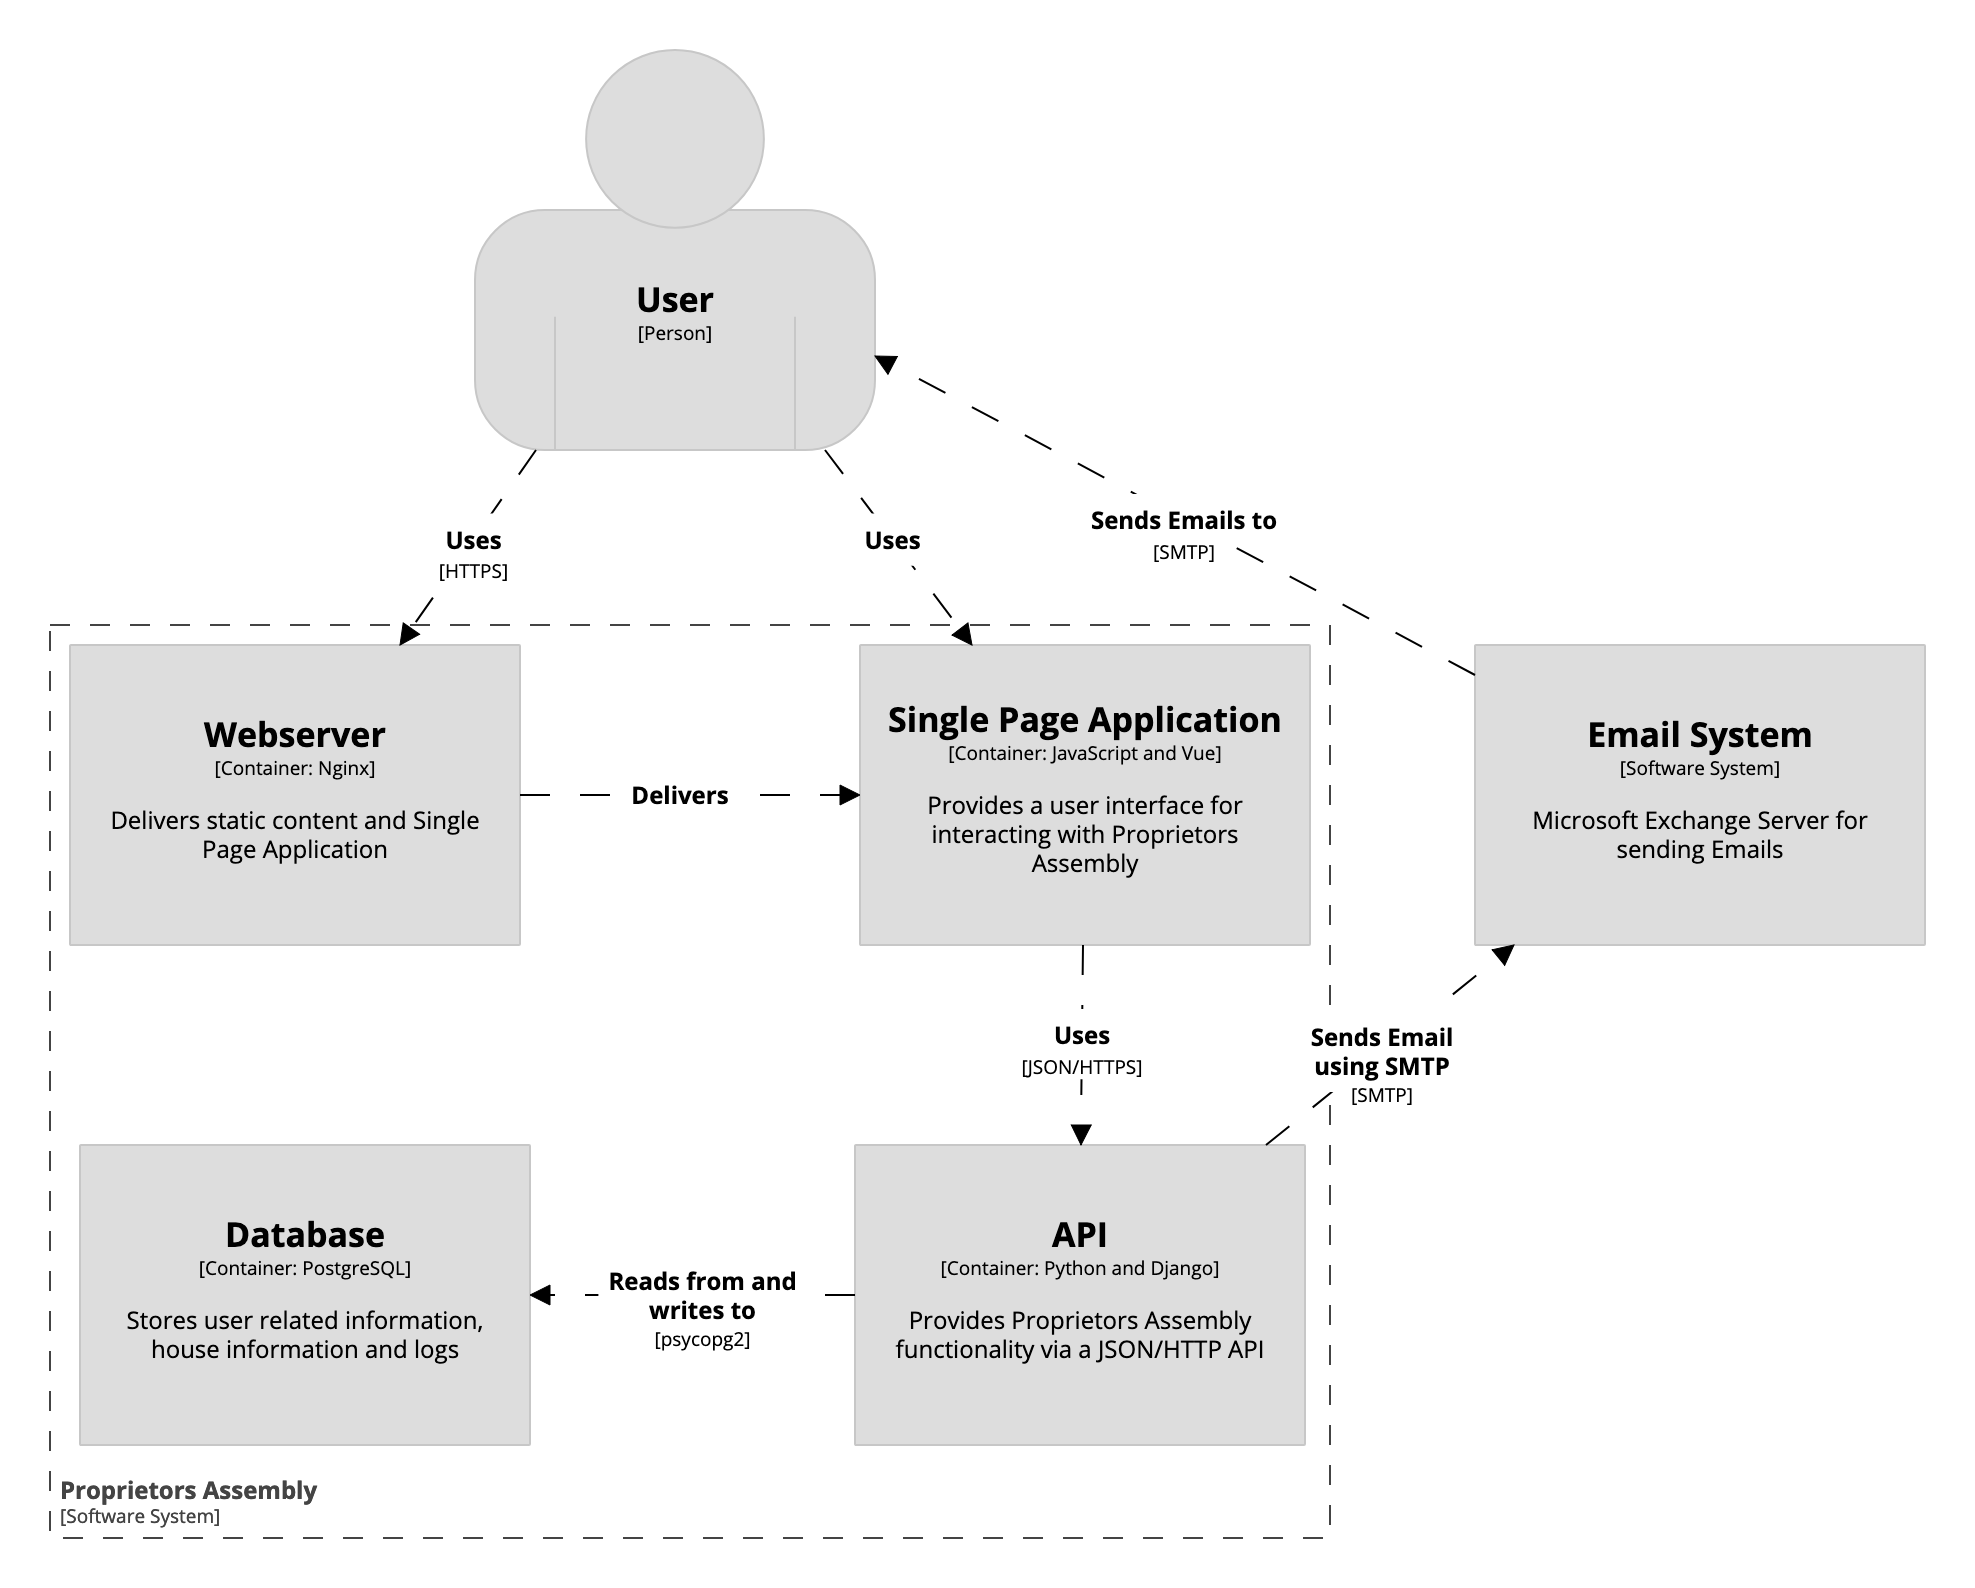
\includegraphics[height=5in]{container_diagram}
    \end{center}
    \caption{System Design}
    \label{fig:usecases}
\end{figure}

Proprietors Assembly as a software system consists of an NGINX web server, the \acrlong{spa}, an API and a database. An external Email System is used by the API to send users emails regarding.

\section{User Interface Design}
Defining how to framework should look like, dashboard-like look, what pages have to be created in order to fullfill requirements. Maybe additional wireframes

\section{Summary}